\subsection{Dữ liệu huấn luyện và tiền xử lý}

Ba mô-đun trong hệ thống sử dụng ba kiểu dữ liệu khác nhau: video RGB cho tầng nhận diện,
chuỗi gloss -- câu tiếng Việt cho tầng ghép câu, và cặp câu song ngữ Việt -- Lào cho tầng
dịch máy. Vì vậy, phần này không thể chỉ liệt kê tên dataset, mà cần mô tả rõ nguồn dữ liệu,
cách tổ chức mẫu, cách chia tập và các bước tiền xử lý cho từng mô-đun. Đây là cơ sở để người
đọc đánh giá tính hợp lệ của quá trình huấn luyện và thực nghiệm.

\subsubsection{Mô hình pre-trained cho mô-đun nhận diện ký hiệu}

Khác với hai mô-đun NLP phía sau (có quá trình huấn luyện rõ ràng trên dữ liệu riêng), mô-đun nhận
diện ký hiệu sử dụng một mô hình đã được huấn luyện sẵn (pre-trained). Cụ thể, hệ thống tích hợp
mô hình TFLite từ giải pháp đạt giải nhất cuộc thi Kaggle \textit{Google -- Isolated Sign Language
Recognition}.

Dữ liệu huấn luyện gốc của mô hình bao gồm:
\begin{itemize}
    \item 250 từ vựng ký hiệu ASL phổ biến;
    \item dữ liệu landmarks đã được trích xuất bằng MediaPipe Holistic (543 landmarks × 3 tọa độ);
    \item nhiều signer với điều kiện ghi hình đa dạng.
\end{itemize}

\begin{table}[H]
\centering
\caption{Thông tin mô hình pre-trained cho mô-đun nhận diện ký hiệu}
\label{tab:asl250-model-info}
\begin{tabularx}{\textwidth}{|X|c|}
\hline
\textbf{Thuộc tính} & \textbf{Giá trị} \\
\hline
Nguồn mô hình & Kaggle ASL Signs 1st Place Solution \\
\hline
Số lớp từ vựng & 250 \\
\hline
Định dạng mô hình & TensorFlow Lite (.tflite) \\
\hline
Kích thước file & $\sim$11 MB \\
\hline
Đầu vào mỗi frame & 543 landmarks × 3 tọa độ \\
\hline
Sliding window & 16--60 frames \\
\hline
\end{tabularx}
\end{table}

Vì nhóm không tự huấn luyện mô hình này, phần dữ liệu cho mô-đun nhận diện không có
train/validation/test split do nhóm thực hiện. Thay vào đó, các file cần thiết để chạy mô-đun
nhận diện bao gồm:
\begin{itemize}
    \item \texttt{model.tflite}: trọng số mô hình đã huấn luyện;
    \item \texttt{sign\_to\_prediction\_index\_map.json}: bảng ánh xạ giữa tên từ vựng ký hiệu
    và chỉ số đầu ra;
    \item \texttt{realtime\_asl\_250.py}: script suy luận thời gian thực.
\end{itemize}

Đây là một lựa chọn thiết kế có chủ đích: thay vì đầu tư toàn bộ thời gian vào việc tự huấn
luyện một mô hình nhận diện từ đầu (với rủi ro chất lượng không đảm bảo), nhóm lựa chọn tích
hợp một mô hình đã được kiểm chứng qua cuộc thi Kaggle, từ đó tập trung nguồn lực cho các tầng
NLP phía sau.

\subsubsection{Bộ dữ liệu cho mô-đun ghép câu tiếng Việt}

Theo tài liệu kỹ thuật trong \texttt{vsl.pdf}, mô-đun ghép câu được huấn luyện trên bộ dữ
liệu \textit{VSL Vietnamese NLP Dataset v4 Mega}. Bộ dữ liệu này bao gồm các cặp
\texttt{raw\_sentence} và \texttt{complete\_sentence}, trong đó:
\begin{itemize}
    \item \texttt{raw\_sentence} là chuỗi gloss hoặc chuỗi từ thô được chuẩn hóa từ ngôn
    ngữ ký hiệu;
    \item \texttt{complete\_sentence} là câu tiếng Việt hoàn chỉnh dùng làm nhãn đích.
\end{itemize}

\begin{figure}[H]
\centering
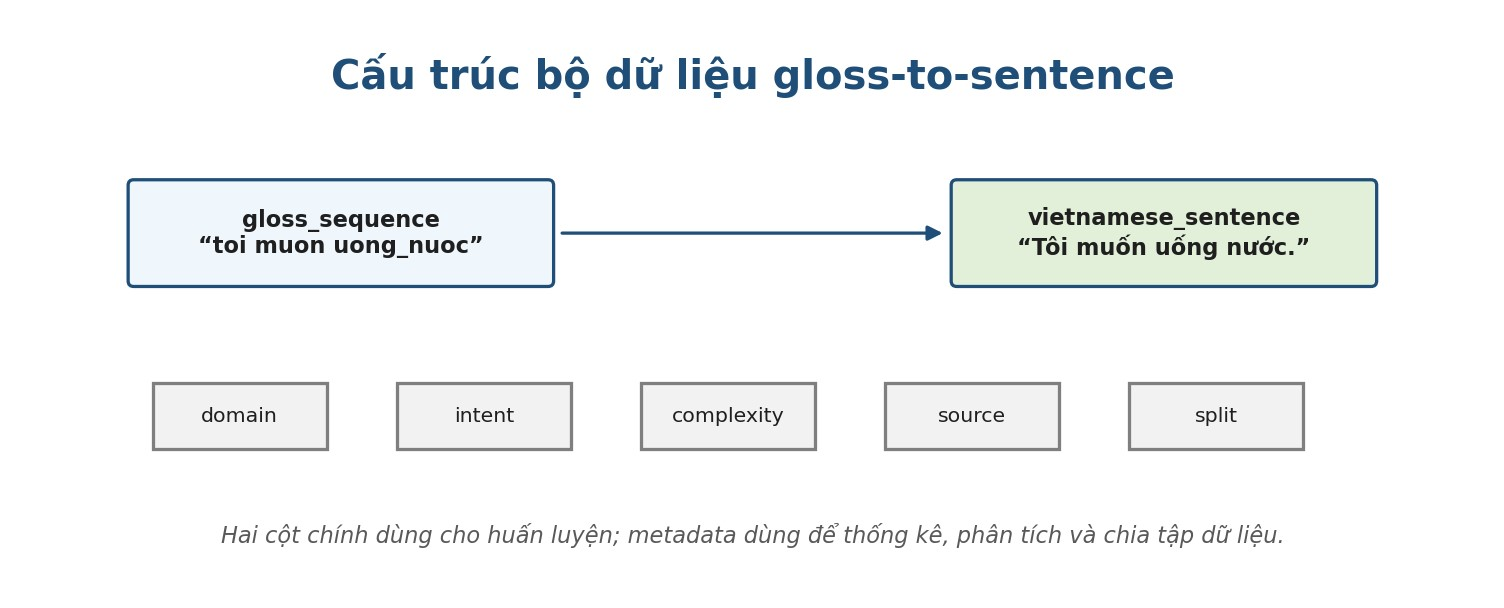
\includegraphics[width=0.82\textwidth]{figures/nlp/vsl_dataset_schema.jpg}
\caption{Cấu trúc một mẫu dữ liệu gloss-to-sentence}
\label{fig:vsl-dataset-schema}
\end{figure}

\begin{table}[H]
\centering
\caption{Thống kê bộ dữ liệu VSL Vietnamese NLP Dataset v4 Mega}
\begin{tabularx}{\textwidth}{|X|c|}
\hline
\textbf{Thuộc tính} & \textbf{Giá trị} \\
\hline
Tổng số mẫu câu & 32.755 \\
\hline
Số gloss token & 262 \\
\hline
Số nhóm ngữ cảnh & 32 \\
\hline
Train set & 26.204 \\
\hline
Validation set & 3.275 \\
\hline
Test set & 3.276 \\
\hline
\end{tabularx}
\end{table}

Bên cạnh bộ dữ liệu đầy đủ được mô tả trong tài liệu, snapshot mã nguồn hiện tại chỉ giữ
lại một tệp \texttt{data/sentence\_pairs.csv} gồm 50 dòng mẫu để phục vụ việc kiểm thử
tích hợp và minh họa cục bộ. Điều này cho thấy repository đang lưu phần tối thiểu cần cho
demo, còn bộ dữ liệu đầy đủ được quản lý bên ngoài ở giai đoạn huấn luyện chính thức.

\begin{figure}[H]
\centering
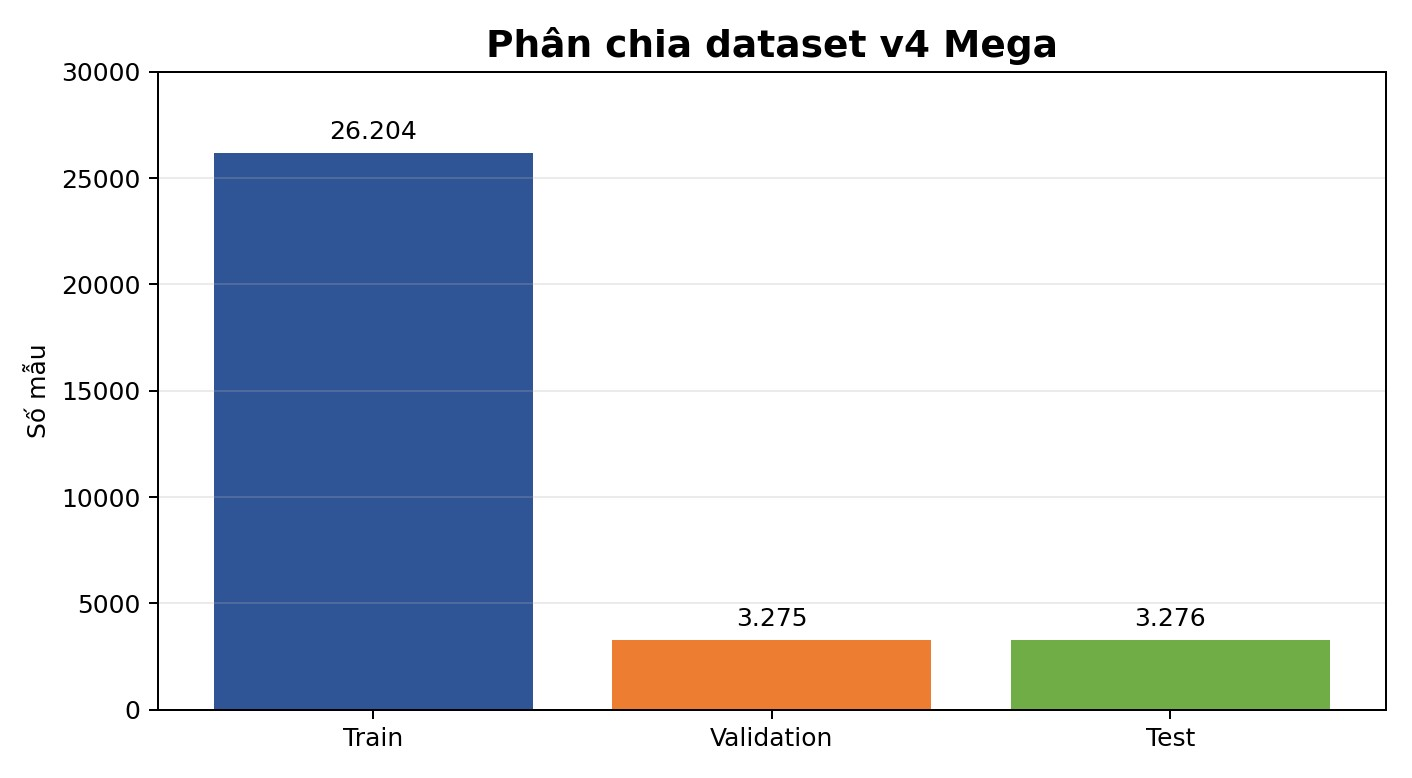
\includegraphics[width=0.82\textwidth]{figures/nlp/vsl_dataset_bar_split.jpg}
\caption{Số lượng mẫu trong các tập train, validation và test}
\label{fig:vsl-dataset-split}
\end{figure}

\begin{figure}[H]
\centering
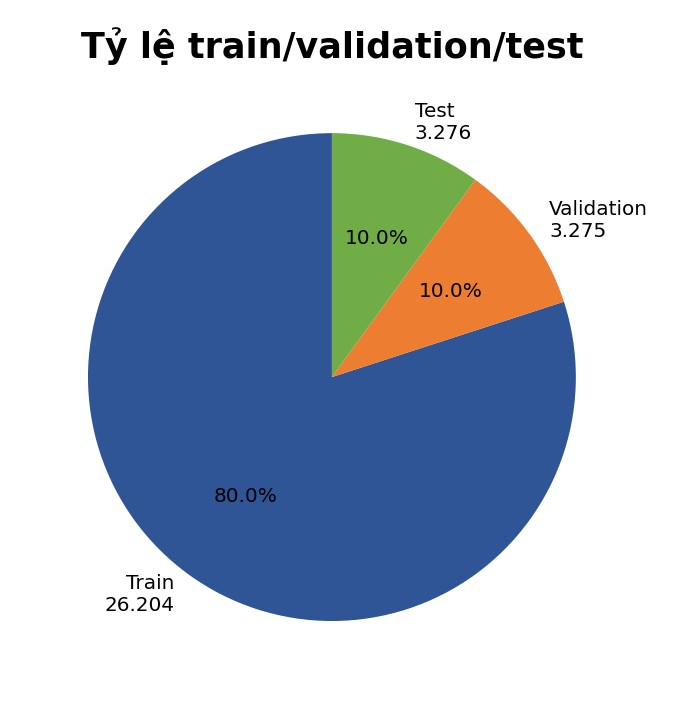
\includegraphics[width=0.55\textwidth]{figures/nlp/vsl_dataset_pie_split.jpg}
\caption{Tỷ lệ chia dữ liệu train, validation và test}
\label{fig:vsl-dataset-pie-split}
\end{figure}

\subsubsection{Tiền xử lý cho mô-đun ghép câu}

Tiền xử lý của mô-đun ghép câu được thực hiện theo đúng bản chất của dữ liệu gloss:
\begin{itemize}
    \item loại bỏ dòng rỗng hoặc giá trị \texttt{NaN};
    \item chuẩn hóa khoảng trắng đầu cuối và khoảng trắng thừa giữa các token;
    \item giữ lại các cụm từ ghép bằng dấu gạch dưới như \texttt{uong\_nuoc},
    \texttt{giup\_do}, \texttt{benh\_vien} để không làm mất đơn vị ý nghĩa;
    \item thêm tiền tố tác vụ \texttt{chuyen\_cau\_ky\_hieu:} vào đầu vào khi train và
    inference;
    \item token hóa bằng tokenizer của \texttt{vinai/bartpho-word-base};
    \item giới hạn độ dài đầu vào và đầu ra ở mức 64 token.
\end{itemize}

Việc giữ nguyên cấu trúc token dạng gloss là rất quan trọng. Nếu tách sai các cụm
\texttt{uong\_nuoc} hoặc \texttt{nha\_ve\_sinh}, mô hình sẽ phải học lại quan hệ ngữ nghĩa
phức tạp hơn và giảm tính ổn định trong quá trình sinh câu.

\subsubsection{Bộ dữ liệu cho mô-đun dịch Việt - Lào}

Tài liệu \texttt{vilo.pdf} mô tả dữ liệu dịch ở quy mô khoảng 100k câu song ngữ. Kiểm tra
thực tế trong repository hiện tại cho thấy thư mục
\codepath{dich-vi_lo/dataset/vi_lo_dataset_split} đã được chia sẵn thành ba tệp
\texttt{train.csv}, \texttt{valid.csv} và \texttt{test.csv}, với hai cột \texttt{vi} và
\texttt{lo}. Số lượng cụ thể như sau:

\begin{table}[H]
\centering
\caption{Thống kê dữ liệu song ngữ Việt - Lào trong repository}
\begin{tabularx}{\textwidth}{|X|c|}
\hline
\textbf{Thành phần} & \textbf{Số câu} \\
\hline
Train set & 90.000 \\
\hline
Validation set & 5.000 \\
\hline
Test set & 5.000 \\
\hline
Tổng số cặp câu & 100.000 \\
\hline
\end{tabularx}
\end{table}

Quan sát nhanh trên các mẫu dữ liệu cho thấy tập song ngữ này khá đa miền: có câu hội
thoại đời thường, câu kể, câu mô tả, tên riêng và câu văn dài. Đây là ưu điểm về độ phủ,
nhưng đồng thời cũng tạo ra thách thức vì dữ liệu có thể chứa nhiễu ở tên riêng, viết hoa,
phiên âm hoặc các cấu trúc câu không đồng đều.

\begin{figure}[H]
\centering
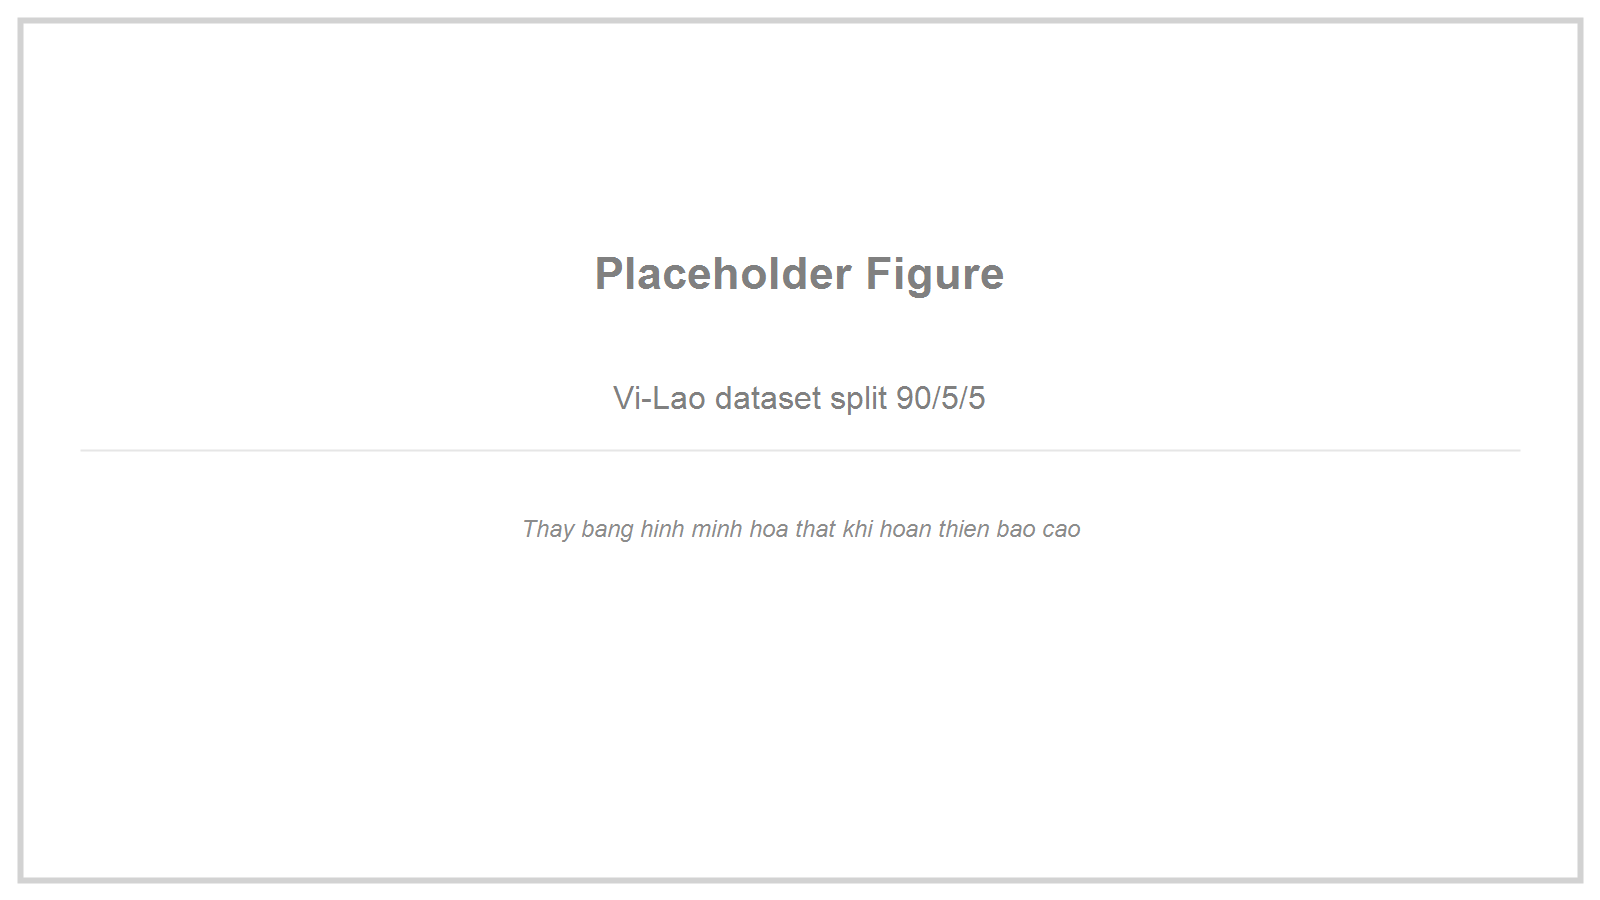
\includegraphics[width=0.82\textwidth]{figures/translation/translation_dataset_split.png}
\caption{Tỉ lệ chia bộ dữ liệu song ngữ Việt -- Lào}
\label{fig:vi-lao-dataset-split}
\end{figure}

\subsubsection{Tiền xử lý cho mô-đun dịch Việt - Lào}

So với mô-đun ghép câu, tiền xử lý của mô-đun dịch tập trung nhiều hơn vào tokenizer đa
ngôn ngữ của NLLB. Trong bản hiện thực hiện tại, các bước chính có thể tóm tắt như sau:
\begin{itemize}
    \item dữ liệu đã được tách sẵn theo câu trong các tệp CSV;
    \item cột nguồn là tiếng Việt, cột đích là tiếng Lào;
    \item tokenizer của NLLB gắn mã ngôn ngữ nguồn \texttt{vie\_Latn} và ngôn ngữ đích
    \texttt{lao\_Laoo};
    \item mô hình sử dụng token hóa kiểu subword của NLLB để giảm vấn đề từ ngoài từ
    điển;
    \item khi suy luận, mô hình được ép bắt đầu bằng token ngôn ngữ tiếng Lào để tránh
    sinh nhầm ngôn ngữ đích.
\end{itemize}

Trong thực nghiệm sau này, nếu cần nâng chất lượng mô hình, hai hướng tiền xử lý nên ưu
tiên là: làm sạch tên riêng và thống nhất quy tắc viết hoa, dấu câu trên cặp dữ liệu song
ngữ. Đây là hai nguồn nhiễu dễ gặp nhất trong tập dữ liệu quan sát được tại thời điểm viết
báo cáo.

